\documentclass{standalone}

\usepackage{tikz}
\usetikzlibrary{fit,calc}
\tikzset{
-latex,
Label/.style={fill=white,sloped,draw,rounded corners,font=\tiny}
}

\newcommand{\MakeStruct}[4][]{%
	\begin{scope}[name prefix = #2@,#1]%
		\edef\tmp{(name)}%
		\node[anchor=north west] (name) at (#3) {\textbf{#2}};%
		\if\relax\detokenize{#4}\relax%
		\else%
			\foreach \t [remember=\t as \prevt (initially name)] in {#4}{%
				\node[anchor=mid west] (\t) at (\prevt.mid east) {\t};%
				\xdef\tmp{\tmp (\t)}%
			}%
		\fi%
		\node[draw,fit=\tmp] (struct) {};%
	\end{scope}%
}

\begin{document}
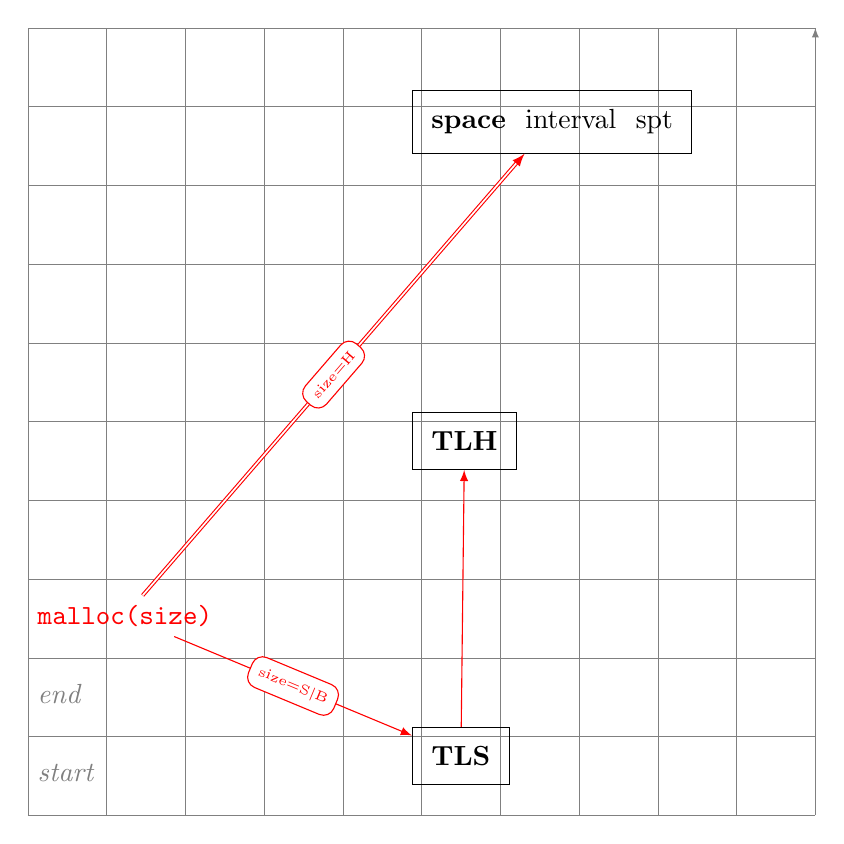
\begin{tikzpicture}
	\draw[help lines] (0,0) grid (10,10);
	
	\begin{scope}[shift={(5,1)}]% Structures
		\MakeStruct{TLS}{0,0}{}
		\MakeStruct{TLH}{0,4}{}
		
		\MakeStruct{space}{0,8}{interval,spt}
	\end{scope}
	
	\begin{scope}[red,yshift=0.5cm]
		
		\begin{scope}[gray]
			\node[anchor=mid west] (ProcessStart) at (0,0) {\textit{start}};
		\end{scope}
		
		\begin{scope}[gray]
			\node[anchor=mid west] (ProcessEnd) at ($(ProcessStart.mid west)+(0,1)$) {\textit{end}};
		\end{scope}
		
		\node[anchor=mid west] (Malloc) at ($(ProcessEnd.mid west)+(0,1)$) {\texttt{malloc(size)}};
		\begin{scope}
			\draw (Malloc) -- node[Label] {size=S$\mid$B}  (TLS@struct);
			\draw (TLS@struct) -- (TLH@struct);
		\end{scope}
		\begin{scope}[every path/.style={double}]
			\draw (Malloc) -- node[Label] {size=H}  (space@struct);
		\end{scope}
	\end{scope}
	

\end{tikzpicture}
\end{document}
